\documentclass{article}



\usepackage{amsmath,amssymb,graphicx,geometry,caption}
\usepackage{xepersian}

\setlength{\parindent}{0mm}




\begin{document}

\large

\begin{center}
به نام او

پایان ترم سیگنال ها و سیستم ها

زمان: 2 ساعت

\hrulefill
\end{center}

سوال 1) اگر سیگنال 
$
x[n]
$
 متناوب با دوره‌ی تناوب اساسی $N$ و ضرایب سری فوریه‌ی آن
$
a_k
$
باشد، در این صورت ضرایب سری فوریه‌ی سیگنالهای زیر را به دست آورید.

\begin{table}[h]
\begin{tabular}{cc}
الف) 
$
y_1[n]=(-1)^nx[n]
$
&
\hspace{25mm}
ب)
$
y_2[n]=\begin{cases}
x[n]&,\quad \text{$n$ زوج}\\
0&,\quad \text{$n$ فرد}
\end{cases}
$
%&
%\hspace{25mm}
%پ)
%$
%\frac{1}{2\pi}\int_{-\pi}^{\pi}|X(e^{j\omega})|^2e^{j\omega}d\omega
%$
\end{tabular}
\end{table}

\hrulefill

سوال 2) اطلاعات زیر در خصوص یک سیگنال گسسته‌ی متناوب
$
x[n]
$
با ضرایب سری فوریه‌ی 
$
a_k
$
داده شده است:

\begin{itemize}
\item
$x[1]=x[3]+2$
\item
$a_k=-a_{k+2}$
\item
$a_2=-1$
\end{itemize}
در این صورت، سیگنال
$
x[n]
$
را بیابید.

\hrulefill

سوال 3) سیگنال 
$
x[n]=1+(-1)^n+e^{j\frac{\pi}{2}n}
$
وارد سیستمی با پاسخ فرکانسی زیر می‌شود:

\begin{figure}[h]
\centering
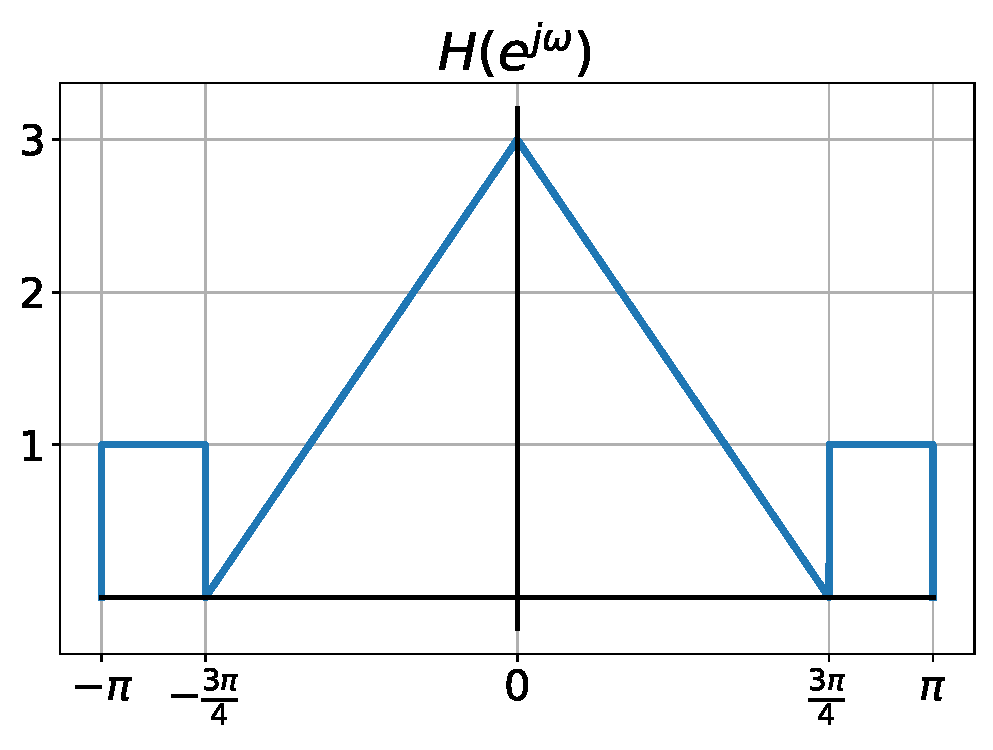
\includegraphics[width=80mm]{Final-Q2.eps}
\end{figure}
خروجی این سیستم را بیابید.

\newpage

سوال 4) سیگنال 
$
x[n]
$
به صورت زیر است:
\begin{figure}[h]
\centering
\includegraphics[width=80mm]{Final-Q3.eps}
\captionsetup{labelformat=empty}
\caption{
سایر نمونه های سیگنال صفرند.
}
\end{figure}

مقادیر زیر را بیابید:
\begin{table}[h]
\begin{tabular}{ccc}
الف) 
$
X(e^{j\pi})
$
&
\hspace{25mm}
ب)
$
\int_{-\pi}^{\pi}X(e^{j\omega})d\omega
$
&
\hspace{25mm}
پ)
$
\frac{1}{2\pi}\int_{-\pi}^{\pi}|X(e^{j\omega})|^2e^{j\omega}d\omega
$
\end{tabular}
\end{table}

\hrulefill

سوال 5) سیستم خطی، مستقل از زمان و پایدار با تابع انتقال
$
H(z)=
\frac{1-3z^{-1}}{\left(1-\frac{1}{2}z^{-1}\right)(1-2z^{-1})}
$
مفروض است.

الف) پاسخ این سیستم به ورودی های 
$
x_1[n]=3^n
$
و
$
x_2[n]=1
$
را در حوزه‌ی زمان بیابید.

ب) پاسخ این سیستم به ورودی
$
x_3[n]=
\left(\frac{1}{2}\right)^nu[n]
+6\cdot 3^nu[-n-1]
$
را در حوزه‌ی زمان بیابید.

پ) پاسخ ضربه‌ی سیستم معکوس را بیابید و پایداری و علی بودن آن را بررسی کنید.
\end{document}